\documentclass{article}
\usepackage{tikz}
\usetikzlibrary{arrows.meta, decorations.pathmorphing, positioning}

\begin{document}

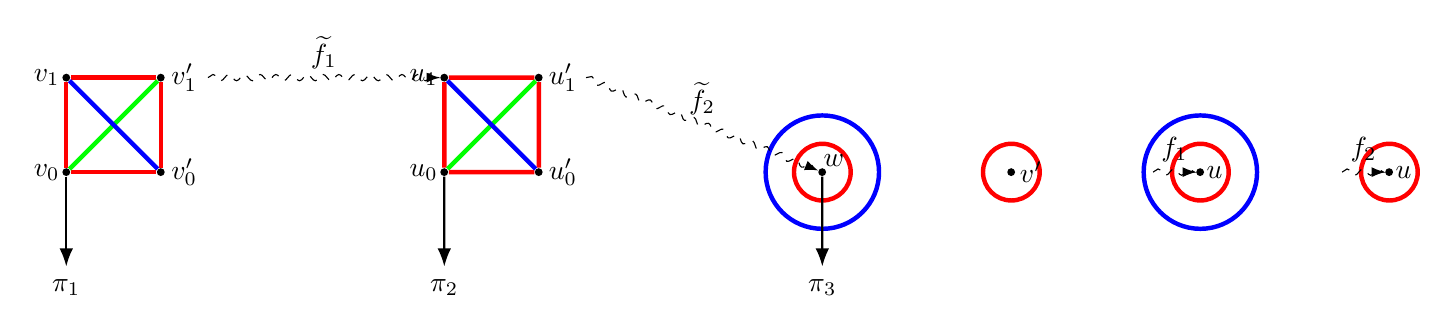
\begin{tikzpicture}[scale=1.2, every node/.style={circle, inner sep=1pt}, >=Latex]

% First Row: Leftmost Graph
\node[fill=black] (v0) at (0,0) {};
\node[fill=black] (v1) at (1,0) {};
\node[fill=black] (v2) at (0,1) {};
\node[fill=black] (v3) at (1,1) {};

\draw[red, ultra thick] (v0) -- (v1) -- (v3) -- (v2) -- (v0);
\draw[green, ultra thick] (v0) -- (v3);
\draw[blue, ultra thick] (v1) -- (v2);

\node[left] at (v0) {$v_0$};
\node[right] at (v1) {$v'_0$};
\node[left] at (v2) {$v_1$};
\node[right] at (v3) {$v'_1$};

% Second Row: Leftmost Graph
\node[fill=black] (u0) at (4,0) {};
\node[fill=black] (u1) at (5,0) {};
\node[fill=black] (u2) at (4,1) {};
\node[fill=black] (u3) at (5,1) {};

\draw[red, ultra thick] (u0) -- (u1) -- (u3) -- (u2) -- (u0);
\draw[green, ultra thick] (u0) -- (u3);
\draw[blue, ultra thick] (u1) -- (u2);

\node[left] at (u0) {$u_0$};
\node[right] at (u1) {$u'_0$};
\node[left] at (u2) {$u_1$};
\node[right] at (u3) {$u'_1$};

% Third Row: Leftmost Graph
\node[fill=black] (w) at (8,0) {};

\draw[red, ultra thick] (w) circle (0.3cm);
\draw[blue, ultra thick] (w) circle (0.6cm);

\node[above right] at (w) {$w$};

% Arrows between left graphs
\draw[->, dashed, decorate, decoration={snake, amplitude=.4mm, segment length=2mm}] 
  (v2) ++(1.5,0) -- node[above] {$\widetilde{f}_1$} (u2) ++(-1.5,0);
\draw[->, dashed, decorate, decoration={snake, amplitude=.4mm, segment length=2mm}] 
  (u2) ++(1.5,0) -- node[above] {$\widetilde{f}_2$} (w) ++(-1.5,0);

% First Row: Rightmost Graph
\node[fill=black] (v_prime) at (10,0) {};
\draw[red, ultra thick] (v_prime) circle (0.3cm);

\node[right] at (v_prime) {$v'$};

% Second Row: Rightmost Graph
\node[fill=black] (u_prime) at (12,0) {};
\draw[red, ultra thick] (u_prime) circle (0.3cm);
\draw[blue, ultra thick] (u_prime) circle (0.6cm);

\node[right] at (u_prime) {$u$};

% Third Row: Rightmost Graph
\node[fill=black] (u_final) at (14,0) {};
\draw[red, ultra thick] (u_final) circle (0.3cm);

\node[right] at (u_final) {$u$};

% Arrows between right graphs
\draw[->, dashed, decorate, decoration={snake, amplitude=.4mm, segment length=2mm}] 
  (v_prime) ++(1.5,0) -- node[above] {$f_1$} (u_prime) ++(-1.5,0);
\draw[->, dashed, decorate, decoration={snake, amplitude=.4mm, segment length=2mm}] 
  (u_prime) ++(1.5,0) -- node[above] {$f_2$} (u_final) ++(-1.5,0);

% Vertical arrows for projections
\draw[->, thick] (v0) --++ (0,-1) node[below] {$\pi_1$} (v_prime);
\draw[->, thick] (u0) --++ (0,-1) node[below] {$\pi_2$} (u_prime);
\draw[->, thick] (w) --++ (0,-1) node[below] {$\pi_3$} (u_final);

\end{tikzpicture}

\end{document}